% Created 2020-01-06 lun. 13:42
% Intended LaTeX compiler: pdflatex
\documentclass[review, 3p]{elsarticle}
\usepackage[utf8]{inputenc}
\usepackage[T1]{fontenc}
\usepackage{graphicx}
\usepackage{grffile}
\usepackage{longtable}
\usepackage{wrapfig}
\usepackage{rotating}
\usepackage[normalem]{ulem}
\usepackage{amsmath}
\usepackage{textcomp}
\usepackage{amssymb}
\usepackage{capt-of}
\usepackage{hyperref}
\usepackage{color}
\usepackage[english]{babel}
\usepackage[matha,mathb]{mathabx}
\usepackage{amsmath}
\usepackage{lineno}
\usepackage{hyperref}
\journal{Journal of Archaeological Science: Reports}
\modulolinenumbers[1]
\bibliographystyle{model5-names}\biboptions{authoryear,sort}
\newcommand{\med}{\text{med}}
\date{\today}
\title{}
\hypersetup{
 pdfauthor={Frédéric Santos},
 pdftitle={},
 pdfkeywords={},
 pdfsubject={},
 pdfcreator={Emacs 26.3 (Org mode 9.3.1)}, 
 pdflang={English}}
\begin{document}


\begin{frontmatter}

\title{An overview of some robust methods for univariate and multivariate outliers detection with applications to archaeological samples}

\author{Frédéric Santos\corref{cor1}}
\ead{frederic.santos@u-bordeaux.fr}
\cortext[cor1]{Corresponding author}
\address{Université de Bordeaux, UMR 5199 PACEA, Bâtiment B8, Allée Geoffroy Saint-Hilaire, CS 50023, 33615 Pessac Cedex, France.}

\begin{abstract}
Whereas outlier detection is routinely performed in archaeological sciences and may have a substantial impact of subsequent discussion and interpretations, modern and robust methods are rarely employed in our disciplinary field. The detection of univariate outliers mainly relies on the well-known rule of ``sample mean plus or minus two standard deviations'', whose the lack of robustness is illustrated in this article. Furthermore, specific and efficient methods for multivariate outliers seem to be very little known and rarely used through the literature published in the \textit{Journal of Archaeological Science: Reports}. To fill this gap, this article aims to present and summarize some robust methods well suited to the data usually gathered in archaeological and anthropological sciences, for both univariate and multivariate outliers. Robust methods for correlation and linear regression, whose results remain correct even in presence of strong outliers, are also illustrated. Methodological guidelines are discussed, in the light of applications on osteometric data extracted from the Goldman Data Set online. All the results (figures and tables) presented in this article can be fully reproduced with the companion R code available online, thus providing to the researchers some examples of templates for outliers detection.
\end{abstract}

\begin{keyword}
isolation forests \sep MAD \sep robust Mahalanobis distance \sep robust statistics \sep R language
\end{keyword}

\end{frontmatter}

\linenumbers
\section{Introduction}
\label{sec:orgeed441b}
According to the intuitive definition formulated by \citet[p.1]{hawkins1980_IdentificationOutliers}, an outlier is ``\emph{an observation which deviates so much from other observations as to arouse suspicions that it was generated by a different mechanism}''. Detecting outliers is an important step, either upstream of statistical analyses or as a goal in its own right. Some outliers may be due to various sources of error such as entry errors, strong measurement errors, or artifacts that may arise at different steps of data acquisition in virtual anthropology. But some outlying values may also reveal ``true'' anomalies in the data, and then bring important and relevant information, for they can contribute to identify pathological individuals \citep{dietmeier2018_OxenOxonHill} or individuals having too unusual values to be part of a given human group. The latter case is particularly frequent in isotopic studies where outliers for \(\delta{}^{13}C\), \(\delta{}^{15}N\) or \(\delta{}^{18}O\) values might indicate the presence of non-local individuals, thus allowing to discuss migrations and mobility patterns among human groups \citep{santana-sagredo2015_IsotopicEvidenceDivergent,hakenbeck2010_DietMobilityEarly,knudson2011_InvestigatingRegionalMobility,kendall2013_MobilityMortalityMiddle}. Outliers detection can thus have important consequences on subsequent interpretations.

When no pre-existing data providing a range of credible values for a given population can be used---which is the general case in archaeological sciences---, this range of credible values must be estimated with statistical methods, traditionally using location and scale estimates calculated on the sample itself, that are supposed to accurately reveal the true parameters of the underlying population. The data used for those calculations thus include the potential outliers, which raises a crucial problem: if those location and scale estimates are non-robust, i.e. strongly influenced by the presence of outliers, they may fall far from the true population parameters, thus invalidating the whole procedure.

The handling of outliers often suffers from several problems and misuses in past sciences. First, the number and identity of outliers may vary depending on the method employed \citep{lightfoot2014_WaterConsumptionIron}. Nonetheless, the method or criterion used to detect and identify outliers is not always explicitly specified in the scientific literature; this lack of precision is also frequent in other disciplinary subfields of social sciences \citep{leys2013_DetectingOutliersNot}. Second, the methods used in the literature are oftenest not robust, and the decision rules used to identify outliers rely either on statistical indicators that are themselves imprecise in the presence of outliers, and/or a normality assumption which is not always clearly met \citep[e.g.,][]{wright2005_IdentifyingImmigrantsTikal,webb2013_ExploringGeographicOrigins}. Third, although a few publications do utilize efficient and specific methods to detect multivariate outliers \citep[e.g.,][]{harris1988_PrincipalComponentsAnalysis,mahoney2006_DentalMicrowearNatufian,algee-hewitt2016_PopulationInferenceContemporary}, numerous articles rely on a combination of univariate methods applied separately on each variable, which is sub-optimal and can even lead to misleading results. Finally, both the modern statistical methods for detecting outliers and their implementation in free software seem to be little known. 

The problem of outlier detection is also closely related to the robustness of statistical methods. Indeed, outliers are often identified ---and sometimes excluded---in search for a more ``representative'' sample to assess and discuss the correlation between two variables \citep[e.g.,][]{loftus2012_TechnicalNoteInterpreting}, or to build regression models \citep[e.g.,][]{beck_DonThrowBaby}. This article will focus on robust methods, both for detecting outliers themselves, and also for getting more precise statistical estimates even when outliers are present in a dataset. Some examples where those robust methods outperform more classical and widely used methods will be given, using population samples extracted from the Goldman Data Set freely available online \citep{auerbach2004_HumanBodyMass}. 

The aim of this article is not to provide an exhaustive or practical in-depth review of all available methods of outlier detection. A comparison of several methods, applied on isotopic data, has recently been performed by \cite{lightfoot2016_UseBiomineralOxygen} in an enlightening article. \cite{leys2019_HowClassifyDetect} recently published a methodological note to ``\emph{fill the lack of an accessible overview of best practices}'' (p. 1) for outliers detection in the field of psychology. However, there is a strong need that a similar dissemination reaches the field of archaeological sciences. For instance---as of september 2019---, a research within the database of the articles published in \emph{Journal of Archaeological Science: Reports} triggered only three results for the keywords ``median absolute deviation'', two results for ``bagplot'', one result for ``robust Mahalanobis'', and no result could be found for requests about ``multivariate outliers'' or the \(S_n\) estimator. As concerns robust methods, the keywords ``robust regression'' or ``quantile regression'' triggered one single result---which furthermore only deals with local polynomial regression (LOESS). Those results are nearly identical---and sometimes even lower---in other journals more oriented towards biological anthropology, such as the \emph{American Journal of Physical Anthropology} or the \emph{International Journal of Osteoarchaeology}.

Consequently, this article proposes a summary of the recent advances in statistics, illustrates some caveats of the most used methods, and provides ready-to-use R templates for modern methods of outlier detection. Several excellent R packages already provide useful functions implementing the robust methods described in this article, such as \texttt{Routliers} \citep{klein2019_RoutliersRobustOutliers} or \texttt{univOutl} \citep{dorazio2018_UnivOutlDetectionUnivariate}. Some additional functions, mainly bringing more options of data vizualisation, are implemented in an R package introduced in the present article, \texttt{anthrostat}, which is available on GitLab (\url{https://gitlab.com/f.santos/anthrostat}).

Finally, to reinforce the move towards a reproducible research in archaeological and anthropological sciences \citep{marwick2017_ComputationalReproducibilityArchaeological,marwick2017_OpenScienceArchaeology}, this whole article has been written in Org-mode 9.3.1 for Emacs 26.3 \citep{schulte2012_MultiLanguageComputingEnvironment,stanisic2015_EffectiveGitOrgMode} and is fully reproducible with the org source file available on GitLab (\url{https://gitlab.com/f.santos/reproducibility-package-for-santos-2020-jasr}). For non Emacs users, the source code of all tables and figures from this study has also been made available in separate R files. All the statistical analyses were performed with R 3.6.2 \citep{rcoreteam2019_LanguageEnvironmentStatistical}.

\section{Univariate outliers}
\label{sec:org6cd6a96}
This first section deals with outlying values for one sigle variable. To present a concrete archaeological case, the left-right differences in humerus maximum length observed on the hunter-gatherers of Ipituaq (US-AK, 1500--1100 BP) are used. Those data are extracted from the Goldman Data Set online. This population sample is known to exhibit a substantial amount of asymmetry for this measurement \citep{auerbach2008_PatternsClavicularBilateral}. Since significant sex differences may be observed on the upper limbs for forager populations \citep{weiss2009_SexDifferencesHumeral}, only the 14 male individuals whose humeral length is known on both sides are considered. This small sample also allows to discuss the robustness of the several methods presented below with the sample sizes usually available in archaeological sciences.

\subsection{The classical rule based on the sample mean and standard deviation}
\label{sec:org3f437ab}
In biological anthropology, methods of outlier detection based on the mean and standard deviation are still frequently employed, including in recent research articles \citep[e.g.,][]{bergstrom_NutritionalImportanceInvertebrates,lubritto2017_NewDietaryEvidence}. Any value out of the range defined by the mean plus or minus two or three standard deviation is then considered as an outlier. This criterion, also known as the ``95–99.7 rule'', is derived from the properties of the gaussian distribution: it is well known that about 95\% and 99.7\% of normally distributed values lie within two and three standard deviations from the mean respectively. This rule-of-thumb is both theoretically and practically correct when applied to a large enough sample, for which the assumption of normality seems reasonable.

However, this method suffers from a critical lack of robustness in other situations, recently illustrated on real data from various disciplinary fields by \cite{leys2013_DetectingOutliersNot} and \cite{lightfoot2016_UseBiomineralOxygen}. The data sets handled in past sciences do not always meet the previous requirements, oftenest because of their small sample size. When considering archaeological data, the sample mean and---above all---standard deviation may be drastically distorded by the presence of the extreme outliers themselves, and thus do not provide a good measure of distance to detect outliers.

\begin{figure}[htbp]
\centering
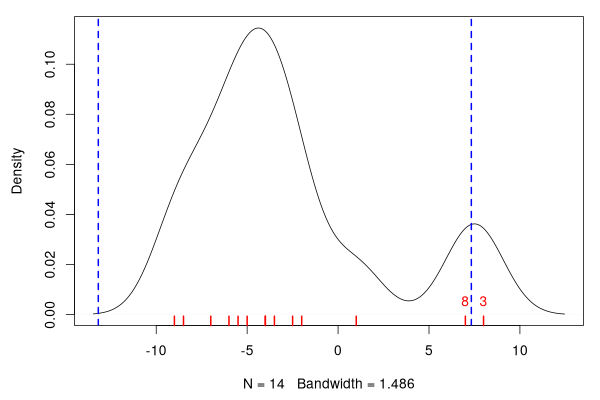
\includegraphics[width=0.6\textwidth]{figures/failure2sd.png}
\caption{\label{fig:org403d450}Kernel density estimation of the vector \(x\) of left-right differences in humeral length observed on the 14 male individuals from the population sample Ipituaq (US-AK, 1500--1100 BP) in the Goldman Data Set. The blue dotted vertical lines represent the exclusion thresholds defined by the classical rule based on the sample mean and standard deviation, equal to \(\bar{x} \pm 2 \times \hat{\sigma}_x\). The third and eight individuals are visual outliers.}
\end{figure}

Figure \ref{fig:org403d450} provides an illustration of such a situation. The sample mean \(\hat{\mu}\) = -2.929 and the standard deviation \(\hat{\sigma}\) = 5.129 are strongly inflated because of the two extreme values located on the right tail. The lack of robustness of the ``mean plus or minus two standard deviations'' decision rule is revealed by the failure to exclude one of the two outliers, since its value falls within the range \([\hat{\mu} - 2 \hat{\sigma}; \hat{\mu} + 2 \hat{\sigma}] =\) [-13.186 ; 7.329].

Albeit not artifical, the example presented here may be seen as peculiar, with a low sample size and two extreme values located on one single tail. However, it shows that this classical rule is clearly non-robust, and should only be used with much precaution and after a careful inspection of the data to ensure that the required assumptions are met.

\subsection{Robust alternatives for gaussian data}
\label{sec:orgca31c46}
If the assumption of a normal \(\mathcal{N}(\mu, \sigma^2)\) distribution of the data---disregarding some potential extreme values---seems to be reasonable for a given variable, several alternatives sharing the same philosophy do exist. All of them consist in using more robust estimates for \(\mu\) and \(\sigma\) than the classical sample mean and standard deviation. Consequently, the estimates calculated to define a ``credible range of variation'' outside of which any value can be considered as an outlier, are themselves fewer sensitive to the presence of outliers, thus always providing a more accurate estimation of the hidden population parameters.

For all the methods detailed in this section, the credible range of variation is defined by the following general formula, perfectly analagous to the ``95-99.7 rule'': 

\begin{equation}
[m - k \cdot \hat{s} \, ; \, m + k \cdot \hat{s}] \label{eq:formula_loc_scale_univ}
\end{equation}

where \(m\) is the sample median---a robust estimate for the expectation \(\mu\)---, and \(\hat{s}\) is a robust estimate for \(\sigma\) \citep{dorazio2017_OutlierDetectionRemarks}. The choice of a constant \(k\), usually lying between \(2\) and \(3\), allows to exclude only clear outliers (if set to a high value, since the interval will be wider) or even slightly suspicious values (if set to a low value, since the interval will be narrower), depending on the goals of the study and the type of data. With very small sample sizes, \(k = 3\) seems recommendable to avoid false positives \citep{leys2019_HowClassifyDetect}.

\subsubsection{The interquartile range}
\label{sec:org52409e3}
The interquartile range (IQR) is defined by the difference between the third and first quartiles of the data. It can be shown that, for a gaussian distribution, \(\hat{s} = IQR / a\), with a scale factor \(a \approx 1.349\), is a consistent estimate of \(\sigma\) \citep{wan2014_EstimatingSampleMean}. Therefore, in this first alternative, the outliers are those extreme values falling outside of the range \([m - k \cdot \frac{IQR}{1.349} \, ; \, m + k \cdot \frac{IQR}{1.349}]\).
\subsubsection{The median absolute deviation}
\label{sec:orgd78e471}
The median absolute deviation (MAD) provides another estimate of \(\sigma\) which is even more robust than the IQR \citep{rousseeuw1993_AlternativesMedianAbsolute}. Although defined more than 40 years ago by \cite{hampel1974_InfluenceCurveIts}, this estimate is still rarely used in archaeological sciences. For a given sample \(x\), the MAD is defined as the scaled median of absolute deviations from the sample median:
\begin{equation}
MAD = b \times \med (|x_i - \med(x)|_{1 \leq i \leq n})  \label{eq:mad}
\end{equation}
The scale factor \(b\) depends on the underlying distribution of the data. If the normality assumption is reasonable (disregarding some potential extreme values), \(b\) should be set to \(1.4826\), which is approximately the opposite of the third theoretical quartile of the distribution \(\mathcal{N}(0,1)\). With this method, the outliers are defined as those values that fall outside of the range \([m - k \cdot MAD \, ; \, m + k \cdot MAD]\)

\subsubsection{The \(S_n\) estimator}
\label{sec:orgcd6faef}
A third alternative is provided by the \(S_n\) estimator \citep{rousseeuw1993_AlternativesMedianAbsolute}. \(S_n\) is defined by:
\begin{equation}
S_n = c \cdot \med_i \left\{ \med_j |x_i - x_j| \right\}  \label{eq:sn}
\end{equation}
and is a very robust estimate of the \(\sigma\) parameter of a gaussian distribution if the scale factor \(c\) is set to \(1.1926\). As for the two previous methods, the outliers are defined as those values that fall outside of the range \([m - k \cdot S_n \, ; \, m + k \cdot S_n]\)

\subsubsection{Application to the Goldman Data Set}
\label{sec:orgc851503}
To compare the three robust methods described above with the usual ``95-99.7 rule'', all four criteria were applied to the 14 male individuals from the Ipituaq population sample. The results can be found on Table \ref{tab:org3e63403}.

\begin{table}[htbp]
\centering
\begin{tabular}{lrrrrrl}
 & Location & Scale & Coef & Lower bound & Upper bound & Outliers\\
\hline
mean and sd & -2.929 & 5.129 & 2 & -13.186 & 7.329 & 3\\
median and IQR & -4 & 2.78 & 2 & -9.56 & 1.56 & 3, 8\\
median and MAD & -4 & 2.965 & 2 & -9.93 & 1.93 & 3, 8\\
median and \(S_n\) & -4 & 3.578 & 2 & -11.156 & 3.156 & 3, 8\\
\end{tabular}
\caption{\label{tab:org3e63403}Comparison of four methods based on location and scale parameters for outlier detection, applied on the data described in Figure \ref{fig:org403d450}. ``Coef'' is the user-defined constant \(k\) used for the construction of intervals, see equation \eqref{eq:formula_loc_scale_univ}. The lower and upper bounds of the intervals built with each method are indicated in the corresponding columns.}

\end{table}

It can be seen that, unlike the usual method based on non-robust estimates, the three robust methods detect both the individuals 3 and 8 as outliers. None of them suffer from the inflation of location and scale parameters---caused by the two outliers located on the right tail---that affects the usual method. As a consequence, at any given value of \(k\), the interval they provide for outlier detection is much narrower, and more accurately captures the range of usual values for the humeral asymmetry in this population sample.

\subsection{Robust methods for non-gaussian data}
\label{sec:orgee27047}
In most contexts of past sciences, such as osteometric or isotopic studies, there is almost always a strong presupposition of normality for all the variables considered---once again, discarding a few potential ``true'' outliers (e.g., migrants, pathological individuals or entry errors). As noted by \citet[][p. 22]{lightfoot2016_UseBiomineralOxygen}, skewed data may simply indicate a sample with several outliers on the same distribution tail, as in Figure \ref{fig:org403d450}. 

Severely skewed distributions arise almost systematically in some disciplinary fields such as neurosciences \citep{rousselet2019_ReactionTimesOther}. Specific methods have been proposed for such variables, and numerous formulas do exist depending on the degree of skewness observed on the data \citep{hubert2008_AdjustedBoxplotSkewed}. Conversely, few variables studied by biological anthropologists or archaeologists are intrinsically far from normality. For those reasons, the need of specific methods for non-gaussian data is lower than in other disciplines. Consequently, the methods accounting for skewed distributions are to be used with caution, for they might lead to spurious results as it will be shown below.

As a general rule:
\begin{enumerate}
\item If the distribution may at least be considered as symmetrical, the previous rules based on the MAD and \(S_n\) estimator remain valid, albeit more difficult to use since their scale factors must be approximated through computer simulations \citep{rousseeuw1993_AlternativesMedianAbsolute}.
\item If an asymmetric or skewed distribution is suspected, the use of a robust measure of skewness such as the medcouple \citep{brys2004_RobustMeasureSkewness} might constitute a useful first step. A high medcouple value (close to 1) may indicate that the variable is intrinsically skewed, i.e. exhibits a substantial skewness that is not only due to a few outliers.
\end{enumerate}

In the general case of no particular assumption about the distribution of the, boxplot-based rules are a simple yet efficient way to proceed.

\subsubsection{The classical boxplot rule}
\label{sec:orgf7c5259}
Boxplots \citep{tukey1977_ExploratoryDataAnalysis} are often used to detect univariate outliers. Widely used in past sciences \citep[e.g.,][]{pickard2017_IsotopicEvidenceDietary}, this rule makes no particular assumption about the underlying distribution. The standard boxplot rule does not use one single location estimate and a scale estimate as previous methods. Instead, the credible range of credible values (i.e., the boxplot \emph{fences}) is defined by:

\begin{equation}
[q_1 - k \cdot IQR \, ; \, q_3 + k \cdot IQR] \label{eq:boxplot}
\end{equation}

where \(q_1\) and \(q_3\) are the first and third empirical quartiles respectively. The constant \(k\) is traditionally set to \(1.5\), although more conservative values such as 2 or 3 are also admissible depending on the goals of the study. It should be noted that this interval is centered around the arithmetic mean of \(q_1\) and \(q_3\) (which is usually not equal to the median) and is not symmetrical.

\subsubsection{Adjusted boxplots for skewed distributions}
\label{sec:org817fcdc}
Some amendments to the previous rule have been proposed to achieve a better accuracy for skewed distributions. For slightly skewed distributions, \cite{kimber1990_ExploratoryDataAnalysis} proposed a rule based on so-called semi-interquartile ranges, and defined the following interval:

\begin{equation}
[q_1 - 2k \cdot (m - q_1) \, ; \, q_3 + 2k \cdot (q_3 - m)]  \label{eq:adjusted_boxplot}
\end{equation}
using previous notations, and a value of \(k\) still usually equal to 1.5.

\subsubsection{Application to the Goldman Data Set}
\label{sec:orga8d2337}
An example of visually slightly skewed distribution can be given by considering the asymmetry in tibia mediolateral diameter within the population sample of Giza (Egypt, 4700--4200 BP, shortcode in the Goldman Data Set: ``Pyramiden, Gizeh''). A kernel density estimation of those values is presented in Figure \ref{fig:org47184de}.

\begin{figure}[htbp]
\centering
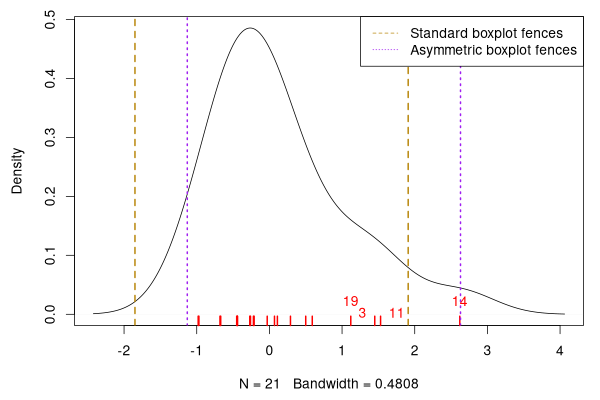
\includegraphics[width=0.6\textwidth]{figures/skewness.png}
\caption{\label{fig:org47184de}Kernel density estimation of the vector right-left differences in tibial mediolateral diameter observed on the 21 individuals from the population sample of Giza (Egypt, 4700--4200 BP) in the Goldman Data Set. The four most extreme individuals on the right tail are labeled in red.}
\end{figure}

Out of any context, this distribution might simply be regarded as right-skewed. Actually, asymmetric boxplot fences do not detect any outlier---not even the extreme individual 14. This basically means that \emph{if one makes the assumption that tibial asymmetries are intrinsically right-skewed in the whole underlying population}, then no value can be regarded as an outlier in this sample. Such an asymmetry pattern might happen: as various subsets of a given population can present different degrees of directional asymmetry \citep{graham2016_FluctuatingAsymmetryHuman}, a complex mixture of fluctuating asymmetry, differential directional asymmetry and/or antisymmetry might indeed end in a skewed distribution. However, if this---strong---assumption is false, accounting for skewness leads to misleading results, since this skewness would not be a characteristic of the underlying population but rather a side-effect of several outliers located on the right tail. Indeed, standard boxplot fences (not adjusted for skewness) do detect the individual 14 as a clear outlier in this population sample.

Accounting for skewed distributions is then a delicate matter and relies on strong biological assumptions that should definitely be supported by previous knwoledge. The choice of a given method of outlier detection must not be based only on statistical considerations, but also depends on the biological knowledge about the variable and population studied \citep{leys2019_HowClassifyDetect}.

\section{Multivariate outliers}
\label{sec:orga619d44}
When several variables are involved, using specific methods is mandatory, and one should not rely on a combination of univariate methods \citep{leys2018_DetectingMultivariateOutliers}. Among other available algorithms such as Dbscan \citep{ester1996_DensitybasedAlgorithmDiscovering}, two methods are detailed below, which are both conceptually rather simple and practically easy-to-use, thanks to very efficient implementations in both R and Python languages.

\subsection{Robust Mahalanobis distance}
\label{sec:orgfddc5ae}
Unlike euclidean distance, Mahalanobis distance takes into account the correlation between the variables when computing dissimilarities among individuals. For this reason, it is popular in biological anthropology \citep{pilloud2016_BiologicalDistanceAnalysis}, where the data suffers almost always from a great intercorrelation. In a formal way, Mahalanobis distance between an individual \(x_i\) (described by \(p\) variables) and the multivariate sample mean \(\hat{\mu}\) is defined by:

\begin{equation}
D_{i} = \sqrt{{}^t(x_i - \hat{\mu}) \Sigma^{-1} (x_i - \hat{\mu})} \label{eq:maha}
\end{equation}

with \(x_i, \hat{\mu} \in \mathbb{R}^p\), and \(\Sigma\) is the \(p \times p\) empirical covariance matrix.

The Mahalanobis distance can be used to detect multivariate outliers \citep[e.g.,][]{stynder2009_CraniometricEvidenceSouth}: the outliers are those individuals whose the distance to the centroid \(\hat{\mu}\) is greater than \(\sqrt{\chi^2_{p; 1-\alpha}}\), i.e. the square-root of the \(1-\alpha\) quantile of a Pearson distribution with \(p\) degrees of freedom. \(\alpha\) may usually vary from 0.001 (for a very conservative rule) to 0.05 (for a not too conservative rule), depending on the aim of the study.

This method is a generalization of the univariate rule relying on the sample mean and standard deviation, described in section \ref{sec:org3f437ab}, and thus it suffers from the same lack of robustness. As for the univariate case, the estimates used in the formula \eqref{eq:maha} are non-robust and may be distorded by potential outliers, thus making invalid the whole decision rule.

A robust variant of Mahalanobis distance was proposed by \cite{hubert2018_MinimumCovarianceDeterminant}. Their method rely on the concept of generalized variance \citep{oja1983_DescriptiveStatisticsMultivariate,wilks1960_MultidimensionalStatisticalScatter,sengupta2006_GeneralizedVariance}, which is a measure of multivariate dispersion defined by the determinant of the covariance matrix, \(|\Sigma|\). The robust Mahalanobis distance proceeds by iteratively drawing at random \(h\) out of the \(n\) individuals (with \(h \in [n/2, n[\)), and finally selecting the subsample of size \(h\) that has the minimum generalized variance. Intuitively, this can be seen as working only on a ``good part'' of the data, i.e. a ``central'' part which does not include the potential outliers. This best subsample of size \(h\) is finally used to compute the sample estimates \(\hat{\mu}_{\text{MCD}}\), \(\hat{\Sigma}_{\text{MCD}}\) that define the robust Mahalanobis distance:

\begin{equation}
R_i = \sqrt{{}^t(x_i - \hat{\mu}_\text{MCD}) \, \hat{\Sigma}_\text{MCD}^{-1} \, (x_i - \hat{\mu}_\text{MCD})} \label{eq:robust_maha}
\end{equation}

This procedure is also known as the MCD (minimum covariance determinant) algorithm. As in the case of the usual Mahalanobis distance, the outliers are defined as those individuals whose robust Mahalanobis distance \(R_i\) exceeds \(\sqrt{\chi^2_{p; 1-\alpha}}\). A study by \cite{leys2018_DetectingMultivariateOutliers} showed that choosing \(h = 3n/4\) should be convenient in most situations, and offers a good compromise between robustness and accuracy.

An implementation of robust Mahalanobis distance is available in the R package \texttt{robustbase} \citep{todorov2009_ObjectOrientedFrameworkRobust}. This package will be used to illustrate the differences between the classical and robust versions of the Mahalanobis distance. Figure \ref{fig:org5a644e9} represents a three-dimensional scatterplot for the Sayala population sample, retrieved from the Goldman Data Set. The maximal lengths of three long bones, the left femur, humerus and tibia, are considered. Visually, three outliers---the individuals 7, 14 and 20---can be identified.

\begin{figure}[htbp]
\centering
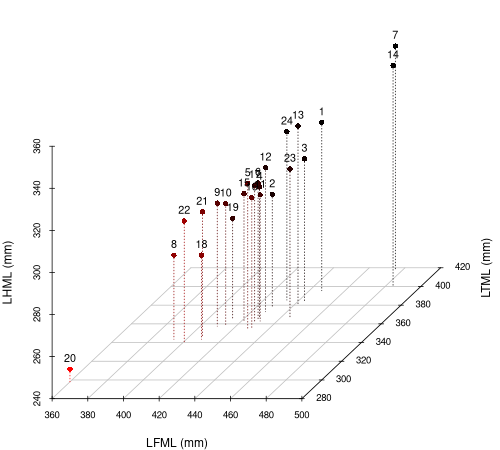
\includegraphics[width=0.55\textwidth]{figures/plot3D-sayala.png}
\caption{\label{fig:org5a644e9}3D scatterplot of the population sample of Sayala, drawn from the Goldman Data Set. The maximal lengths are three long bones are represented.}
\end{figure}

The presence of those outliers causes an inflation of the generalized variance, i.e. the determinant of the classical covariance matrix, \(|\Sigma|\). Consequently, the classical and robust Mahalanobis distances provide different sets of outliers here (Fig. \ref{fig:org30b0333}). For an \(\alpha\) level of 0.01, the classical version detects no outlier at all, whereas the robust version identifies the two individuals 14 and 20. For an \(\alpha\) level of 0.05, the robust version also detects the individual 7, which is still far from the exclusion boundary for the classical version.

\begin{figure}[htbp]
\centering
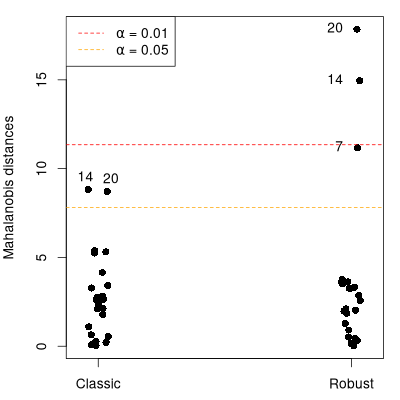
\includegraphics[width=0.45\textwidth]{figures/maha-dd.png}
\caption{\label{fig:org30b0333}Stripcharts displaying the squared classical and robust Mahalanobis distances between each individual and the centroid. The dotted lines symbolize the exclusion thresholds \(\chi^2_{p;1-\alpha}\) for two different \(\alpha\) values. The maximal lengths of three long bones from the population sample of Sayala (Goldman Data Set) were considered (LTML, LHML, LFML).}
\end{figure}

\subsection{{\bfseries\sffamily TODO} Isolation forests}
\label{sec:org2ca74d0}
Isolation forests are a very recent algorithm of ``anomaly detection'' \citep{liu2012_IsolationBasedAnomalyDetection}, based on random forests \citep{breiman2001_RandomForests}. This method does not rely on any assumption about the distribution of the data, nor any given classical dissimilarity (e.g., euclidean, Mahalanobis).

The general idea is that ``anomalies'' can be defined by both their unusual values and their weak number, so that they are quite \emph{isolated} in the data, and therefore easy to localize. Indeed, identifying a point located right in the middle of a point cloud will usually require numerous instructions, whereas one single instruction may be sufficient to describe an outlier (e.g., ``this is the only individual with \(X_5 > 250\)''). 

An isolation forest corresponds to a set of \(B\) \emph{isolation trees}, which are themselves randomly built decision trees that are grown until there is one single individual in each terminal leaf. Since outliers are supposed to be easily isolated in the data, they will correspond to the shortest paths in the isolation trees. A measure of credibility for an individual to be outlier is then its corresponding average path length within the \(B\) isolation trees. An anomaly score, lying in \([0,1]\) and being a function of the sample size and the average path length, is computed for each individual.

According to \cite{liu2012_IsolationBasedAnomalyDetection}, a quick rule-of-thumb can provide a first indication as concerns the presence of outliers: if all the individuals have anomaly scores very close or inferior to 0.5, there is likely no multivariate outlier at all in the data. Conversely, if some anomaly scores depart from 0.5 and raise closer to 1, the corresponding individuals are likely to be outliers.

An isolation forest with 100 isolation trees is built on the same data as in the previous section (Sayala population sample with three variables: LTML, LHML, LFML). The anomaly scores, sorted by decreasing order, can be found in Figure \ref{fig:org5505cf5}. The isolation forest algorithm provides a moderate evidence to consider the individuals 20, 7 and 14 as outliers, since their anomaly scores are the only ones to exhibit a substantial departure from the reference value of 0.50. This conclusion is consistent with the results obtained via the robust Mahalanobis distance (cf. Fig. \ref{fig:org30b0333}). Isolation forests can thus provide a useful indication about possible multivariate outliers, by studying both the global distribution of anomaly scores (in search for ``elbows'' or gaps) and their absolute distance to 0.50.

\begin{figure}[htbp]
\centering
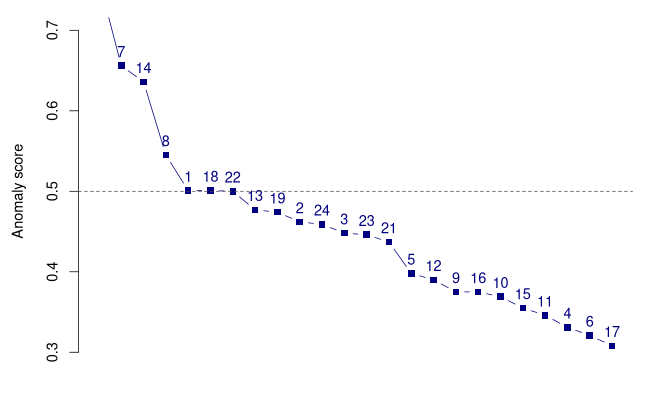
\includegraphics[width=0.6\textwidth]{figures/anomaly_plot.png}
\caption{\label{fig:org5505cf5}Plot of the anomaly scores obtained by an isolation forest to detect outliers from the population sample of Sayala (Goldman Data Set), when three maximal lengths are considered (LTML, LHML, LFML). The scores are sorted in decreasing order and the corresponding individual IDs are indicated.}
\end{figure}

\section{Bivariate outliers}
\label{sec:org96f6bee}
Although the general methods for multivariate outliers detailed in section \ref{sec:orga619d44} can also be used when considering only two variables, some tools were specifically developed for this situation.

\subsection{Outliers in the context of correlation and linear regression}
\label{sec:org82f27cd}
When considering the relationship between two continuous variables, three main types of outliers can be defined. In the first panel of Figure \ref{fig:org2655a96}, one single individual is far from the regression line, but its position---near the average of the explanatory variable RHML---gives it only a limited influence in the regression model. In the middle panel, two extreme individuals can be identified on the margins of the horizontal axis. However, those two individuals perfectly respect the relationship observed on the other individuals, and the regression lines with or withour those two extreme points are indistinguishable. Finally, the right panel shows a \emph{leverage} individual, i.e. an individual which is both located on the margin of the explanatory variable and has a high residual value: this type of individual has a great influence in a regression model, especially when dealing with small sample sizes.

\begin{figure}[htbp]
\centering
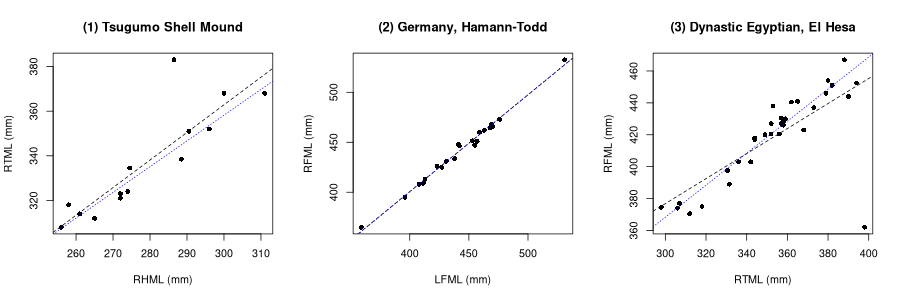
\includegraphics[width=\textwidth]{figures/type_outliers_reg.png}
\caption{\label{fig:org2655a96}Illustration of three types of outliers in linear regression, with three different population samples drawn the Goldman Data Set. Their corresponding shortcodes in this dataset are indicated as the main title; the shortcodes of the variables are indicated as axes labels. The black dotted lines are the regression lines including all the individuals; the blue dotted lines are the regression lines excluding the visual outliers.}
\end{figure}

In a regression model, only the leverage individuals corresponding to the right panel of Figure \ref{fig:org2655a96} are problematic. Leverage individuals can be identified through their high value of Cook's distance, which is provided as a standard diagnostic in most statistical software. A reasonable rule-of-thumb---that should be avoided in the case of a very small sample size---is that leverage points have a Cook's distance greater than 1 \citep{cornillon2010_RegressionAvec}.

However, it should be noted that robust methods for correlation and regression do exist \citep{rousseeuw1987_RobustRegressionOutlier}. Manually excluding outliers is not mandatory with those modern techniques, that have their own built-in way to handle outliers. 

A robust version of the correlation coefficient automatically restricts the computation to the ``most central'' part of the data, using the same MCD algorithm as the robust Mahalanobis distance detailed in section \ref{sec:orgfddc5ae} (Fig. \ref{fig:orgbcf90ca}). In particular, potential outliers can be lefted in on the plots, thus allowing to discuss some particular cases without introducing any bias in the computation.

\begin{figure}[htbp]
\centering
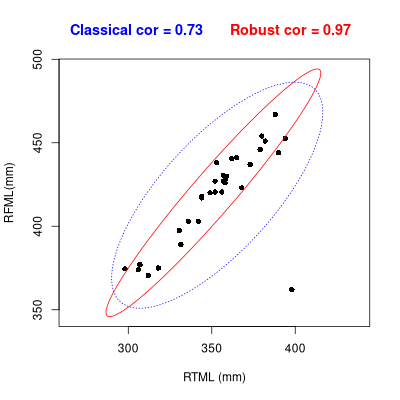
\includegraphics[width=0.5\textwidth]{figures/robust-correlation.png}
\caption{\label{fig:orgbcf90ca}Classical and robust estimates of the correlation coefficient between the maximal lengths of the right humerus and femur within the population sample ``Dynastic Egyptian, El Hesa'' drawn from the Goldman Data Set. Correlation ellipsoids are given an \(\alpha\) level of 0.95, and a proportion \(h=3/4\) of individuals is used for MCD estimation.}
\end{figure}

Robust alternatives for linear regression are also implemented in R. The function \texttt{rlm()} implements an algorithm that gives different weights to the individuals according to their distance to the regression line, and iteratively re-fits the model until convergence \citep{venables2010_ModernAppliedStatistics}. Another option is the quantile regression \citep{koenker2005_QuantileRegressionRoger}, that replaces the mean by the median wihtin the framework of least squares estimation. As shown on Figure \ref{fig:org1ed38d9}, those two methods are usually consistent with each other, and with an ordinary linear regression performed after excluding the potential outliers.

\begin{figure}[htbp]
\centering
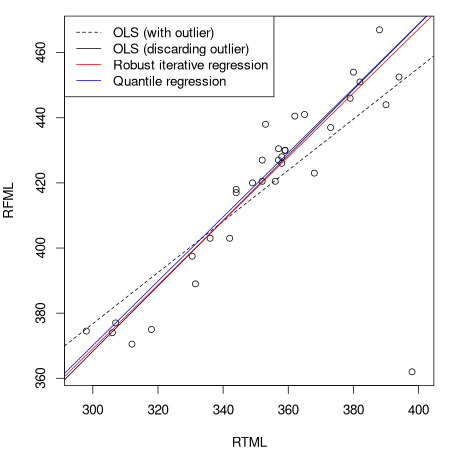
\includegraphics[width=0.5\textwidth]{figures/quantile-regression.png}
\caption{\label{fig:org1ed38d9}Comparison of four strategies of linear regression between the right maximum femur and tibia lengths, using the population sample ``Dynastic Egyptian, El Hesa'' from the Goldman Data Set.}
\end{figure}

\subsection{General case: the bagplot}
\label{sec:org10fb522}
Depending on the aim and context of the study, the two extreme points on the middle panel of Figure \ref{fig:org2655a96} can be seen as clear outliers (they are exceedingly tall and short compared to the other individuals from this population sample) or not (they do respect the relationship between the two measurements). In other words, they are clearly outliers as regards their measurements, but are not outliers in the framework of a regression model.

When one only searches for bivariate outliers outside of the context of linear regression or correlation, the bagplot \citep{rousseeuw1999_BagplotBivariateBoxplot} is the appropriate tool. The bagplot is a bivariate generalization of the boxplot. An inner polygon (\emph{bag}) contains about 50\% of the individuals which are the closest to the bivariate sample median; an exterior \emph{fence} allows to identify the outliers and is defined by inflating the bag by a factor 3; and an intermediate region (the \emph{loop}) is the convex hull of the outermost individuals that are not outliers. Rarely used in archaeological sciences---\cite{oconnell2012_DietbodyOffsetHuman} and \cite{emery2018_MappingOriginsImperial} are two of the few recent instances---, the bagplot provides a simple and visual way to identify bivariate outliers by an \emph{ad-hoc} rule (Fig. \ref{fig:org501e243}).

\begin{figure}[htbp]
\centering
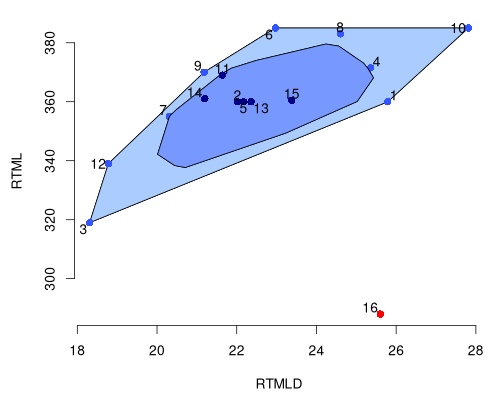
\includegraphics[width=0.6\textwidth]{figures/bagplot.png}
\caption{\label{fig:org501e243}Bagplot for the the maximal length and medio-lateral diameter of the right tibia, measured on the population sample of Delaware (US-NJ, 500 BP) from the Goldman Data Set.}
\end{figure}

\section{Discussion and conclusion}
\label{sec:org2d38802}
As stated by \citet[][p.5]{leys2019_HowClassifyDetect}, ``\emph{there are no universal rules to tell you when to consider a value as ‘too far’ from the others; Researchers need to make this decision for themselves}''. Any method of outlier detection comes from several arbitrary choices from the researcher. The constant \(k\) in equations \eqref{eq:formula_loc_scale_univ} to \eqref{eq:adjusted_boxplot} strongly impact the severity of the decision rule by narrowing or widening the ``credibility intervals''; a similar role is played by the \(\alpha\) level in equations \eqref{eq:maha} and \eqref{eq:robust_maha} for Mahalanobis distances. By chosing lower or higher values for such parameters, either only the clearest extreme values or even slightly unusual values will be regarded as outliers. There is no possibility to give a universal recommendation to set those parameters at a given value, and the researcher should be prepared to defend the strategy of outlier detection adopted in a study.

Furthermore, it is rather unlikely that an archaeologist can know beforehand the distribution of the variable(s) considered in the underlying population. The gaussian distribution, or at least a symmetrical distribution, can be a reasonable assumption in the large majority of situations encountered in past sciences. However, one can almost never know with certainty which distribution a given set of values comes from. In some ambiguous situations (cf. Fig. \ref{fig:org47184de}), the assumptions made by the researcher also greatly impact the results of outlier detection.

For all those reasons, outlier detection is strongly user-dependent, and the strategy adopted should be explicitly stated. One should not rely on vague and non-specific assertions such as ``after removing four outliers, we performed linear regression [\ldots{}]'' without additional details.

The focus of the present article was on outlier detection, and not outlier management in a broad sense. The problem of kwowing what to do with the individuals that are detected as outliers is extensively covered in \cite{leys2019_HowClassifyDetect}. However, numerous robust methods have built-in way to handle outliers, and do not need a controversial manual exclusion. This article focused on robust correlation and regression methods, but most popular methods do have a robust equivalent which offers a valuable alternative for ``contaminated data''. Among other examples, robust principal component analysis \citep{candes2011_RobustPrincipalComponent} or robust estimation and hypothesis testing \citep{wilcox2012_IntroductionRobustEstimation} can be cited. Within the field of robust estimation, winsorization---i.e., replacing all the values exceeding a given threshold \(t\) by the value \(t\) itself---or trimming---i.e., removing a given percentage of the most extreme values in both directions---could be valuable tools in archaeology, and would offer some new ways to deal with outlying values.

\section*{{\bfseries\sffamily TODO} Acknowledgments}
\label{sec:org21fac4e}
\begin{itemize}
\item Reviewers
\item Granger
\item Legrand
\end{itemize}

\section*{{\bfseries\sffamily TODO} Data availability statement}
\label{sec:orgf117676}

\bibliography{../../../../../complete_biblio}
\end{document}